\documentclass[a4paper,11pt]{article} 
% Load some standard packages
\usepackage{amsmath,parskip,fullpage,natbib,graphicx} 

\usepackage{hyperref}

% Deal with multiple figures
\usepackage{subcaption}

% Deal with table rules
\usepackage{booktabs}

% Define my own commands
\newcommand{\info}{{\cal I}}
\newcommand{\E}{\text{E}}

% Bibliography style
\bibliographystyle{agsm}

\begin{document}  
\title{A \LaTeX~Sample}
\author{Yanfei Kang}

\maketitle


\section{Introduction}

Once upon a time there was a lonely honours student, desperate to write
an awesome thesis. She hit upon the idea of making it look beautiful by using a mathematical document preparation system.

\subsection{MS-Word?}
MS-Word may sometimes be useful for short notes or for making a ``Back in 5 minutes" sign to stick on your door, but if you want to write a serious document like an academic paper, a book or a thesis, then you should use a serious tool such as \LaTeX.

\subsection{Who use \LaTeX ?}
LaTeX is not something that would find much use in a corporate office environment. Who is LaTeX for?

\begin{itemize}

\item You -- there is no better software for writing essays, term papers, presentations, and research papers.
\item Grad Students -- I wrote my Master’s thesis in LaTex. I can’t imagine doing anything like that in Word. It would be a suicide. Don’t do it to yourself. Use the proper tool for this task – that tool is LaTeX.
\item Writers -- LaTeX was designed for publishing, and there is no other tool that will produce high quality almost-ready-to-print documents out of your manuscripts.
\item Scientists and Researchers -- no other tool makes it so easy to write research papers, books and journal articles.
\item Professors -- in the past I used LaTeX to generate great looking multiple choice exams, lecture presentation slides, lecture notes and etc.
\item Developers -- you want great looking documentation and user manual? This is the tool for you. LaTeX can also output to HTML so you can easily create googlable online copies of all your documents.
\end{itemize}

\section{Literature review}

In printing, text is emphasized by using \emph{italics}, or possibly using \textbf{bold}.

Footnotes\footnote{This is an example of a footnote.} pose no problem.

A frequently-displayed structure is a list. The following is an example of an \emph{itemized} list.
\begin{itemize}
   \item  This is the first item of an itemized list. You can select other bullet types if you want using additional packages.

   \item  This is the second item of the list.
\end{itemize}
We can also have \emph{enumerated} lists:
\begin{enumerate}
  \item This is the first item of an enumerated list. The numbering of items is automatic. You can enumerate lists with (a), (b), etc., or some other scheme. Using 1., 2., etc., is the default.

  \item This is the second item of the list. 
\end{enumerate}

\section{Figures}


\begin{figure}[h!]
  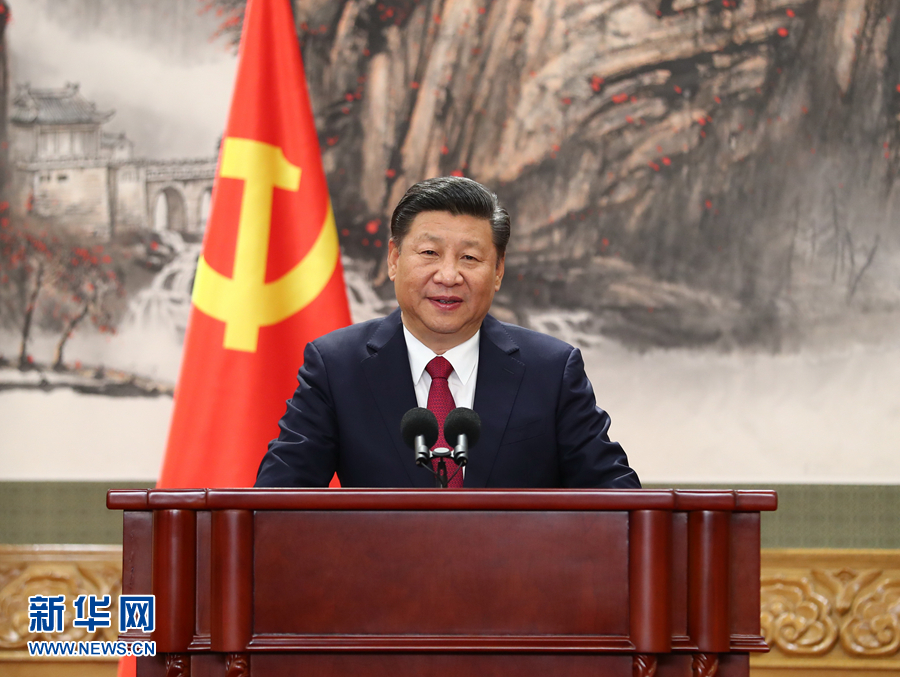
\includegraphics[width=\linewidth]{./figures/19-1.jpg}
  \caption{The general secretary of the CPC central committee.}
  \label{fig:fig1}
\end{figure}

Figure \ref{fig:fig1} shows $\cdots$.

\begin{figure}[h!]
  \centering
  \begin{subfigure}[b]{0.5\linewidth}
    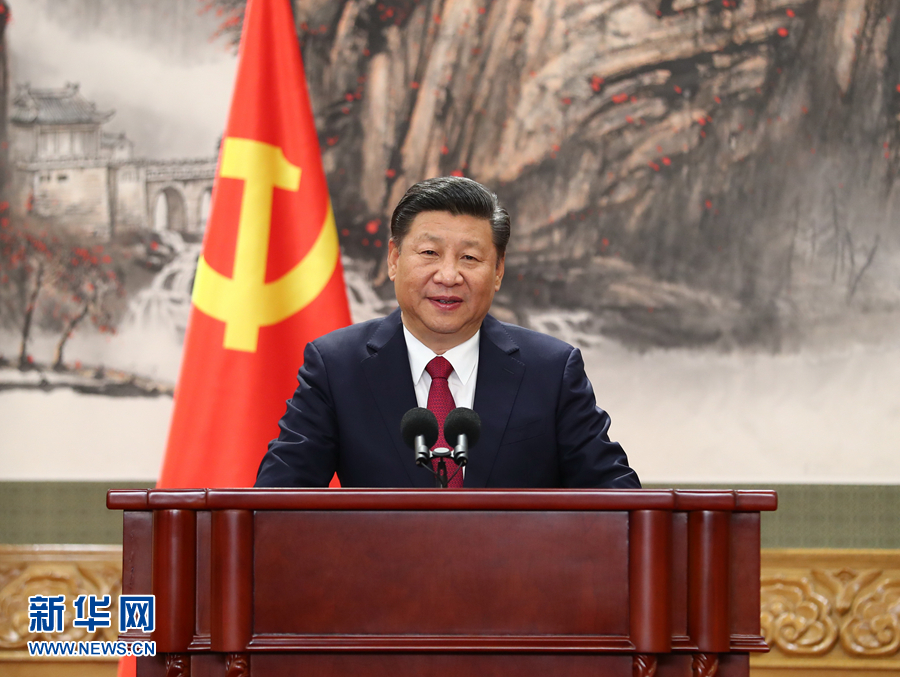
\includegraphics[width=\linewidth]{./figures/19-1.jpg}
    \caption{The general secretary of the CPC central committee.}
  \end{subfigure}
  \begin{subfigure}[b]{0.5\linewidth}
    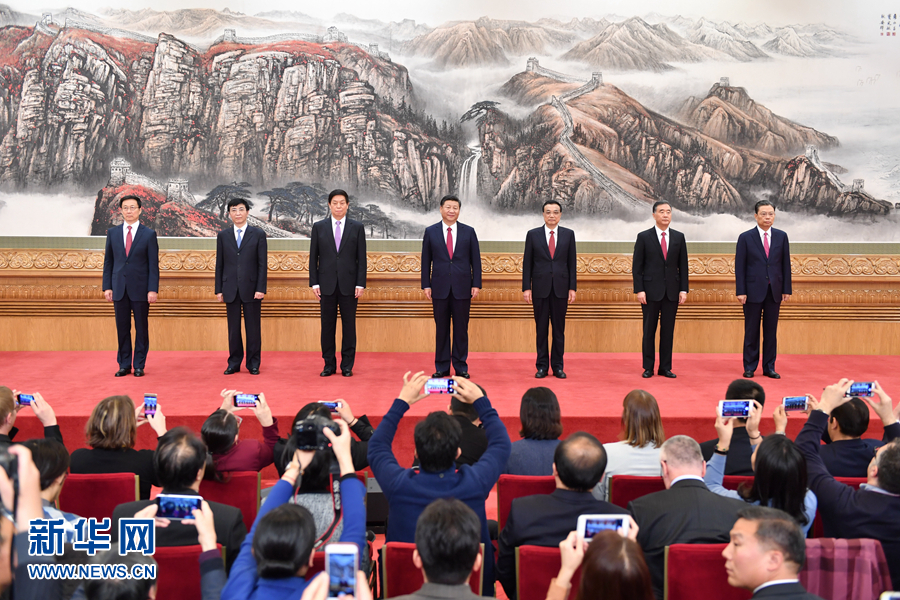
\includegraphics[width=\linewidth]{./figures/19-2.jpg}
    \caption{The standing committee of the CPC central committee.}
  \end{subfigure}
  \caption{Two figures from the 19th CPC National Congress}
  \label{fig:fig2}
\end{figure}

Figure \ref{fig:fig2} shows $\cdots$.

\subsection{Tables}

\begin{table}[h!]
  \centering
  \caption{Caption for the table.}
  \label{tab:table1}
  \begin{tabular}{l|c||r}
    \toprule
    1 & 2 & 3\\
    \hline
    a & b & c\\
    \bottomrule
  \end{tabular}
\end{table}

\section{Mathematics}

For mathematics, wrap symbols in \$ signs. For example, $x-3y=7$
or $a_{1} > x^{2n} / y^{2n} > x' $.
Remember that a letter like $x$ is a formula when it denotes a
mathematical symbol, and should be treated as one.

Mathematical formulas may also be displayed.  A displayed formula
is one-line long; multiline formulas require special formatting
instructions.
$$
  x' + y^{2} = z_{i}^{2}.
$$
Don't start a paragraph with a displayed equation, nor make one a
paragraph by itself.

Numbered equations are also useful:
\begin{equation}\label{eq:mean} 
         \bar{y} = \frac{1}{n} \sum_{i=1}^{n} y_i
\end{equation}
Clearly, equation \eqref{eq:mean} gives the sample mean.  The
sample standard deviation can be calculated similarly:
\begin{equation*}
        s_y = \sqrt{ \frac{1}{n-1} \sum\limits_{i=1}^n (y_i-\bar{y})^2 }.
\end{equation*}

Here \citet{SM86}  is a section from a paper I am writing showing some additional features along with citations. The Poisson model \citep{SM86} is given by
\begin{subequations}\label{HF}
\begin{align}
y_t   &\sim \text{Poisson}(x_{t-1}) \label{HF.1} \\
x_t &= x_{t-1} \eta_{t-1}/\lambda  \label{HF.2}
\end{align}
\end{subequations}
where $\eta_t \sim \text{Beta}(\lambda b_t,(1-\lambda) b_t)$, $b_t=\lambda b_{t-1}+y_t $, and $0<\lambda<1$.  Here we use the Beta$(\alpha,\beta)$ density $f(x) \propto x^{\alpha-1}(1-x)^{\beta-1}$, $0\le x\le1$. Equivalently,
\begin{equation}\label{prodeta}
x_t = \lambda^{-t}x_0\prod_{i=1}^t\eta_i.
\end{equation}
\citet{HF89} show that \eqref{HF} has the EWMA forecast function
\[
  \E(y_{t+h}\mid \info_t) = (1-\lambda)\sum_{j=0}^{t-1} \lambda^j y_{t-j}.
\]




\bibliography{sample}

\end{document} 



